%! TeX program = lualatex
\documentclass[12pt, landscape]{scrartcl}

\usepackage[paperheight=12in,paperwidth=18in,margin=0in,heightrounded,showframe]{geometry}
\usepackage{graphicx}
\usepackage[osf]{libertine}
\usepackage{lettrine}
\usepackage[dvipsnames]{xcolor} 
\usepackage[object=vectorian]{pgfornament}
% \usepackage[document]{ragged2e}
\usepackage{background}
\usepackage{pifont}
\usepackage{soul}

\usetikzlibrary{calc}
\definecolor{fondpaille}{cmyk}{0,0,0.1,0}
\definecolor{calpolypomonagreen}{rgb}{0.12, 0.3, 0.17}
\definecolor{forestgreen(traditional)}{rgb}{0.0, 0.27, 0.13}
\definecolor{darkgreen}{rgb}{0.0, 0.2, 0.13}

\backgroundsetup{
scale=1,
opacity=1,
angle=0,
color=darkgreen,
contents={%

\begin{tikzpicture}[every node/.style={inner sep=0pt}]
\node[anchor=north west](CNW)
at (current page.north west) {\pgfornament[width=4.5cm]{63}};
\node[anchor=north east](CNE)
at (current page.north east) {\pgfornament[width=4.5cm,symmetry=v]{63}};
\node[anchor=south west](CSW)
at (current page.south west) {\pgfornament[width=4.5cm,symmetry=h]{63}};
\node[anchor=south east](CSE)
at (current page.south east) {\pgfornament[width=4.5cm,symmetry=c]{63}};
%
% \node[anchor=north, rotate=0](CNW)  at (current page.north)
% {\pgfornament[width=10cm,symmetry=c]{71}}; 
% \node[anchor=south, rotate=0](CNW)  at (current page.south)
% {\pgfornament[width=10cm,symmetry=c]{71}}; 
%
\node[shift={(5.0cm,0cm)},anchor=north west, rotate=0](CNW)  at (current page.north west)
{\pgfornament[width=10cm,symmetry=c]{71}}; 
\node[shift={(5.0cm,0cm)},anchor=south west, rotate=0](CNW)  at (current page.south west)
{\pgfornament[width=10cm,symmetry=c]{71}}; 
%
\node[shift={(-5.0cm,0cm)},anchor=north east, rotate=0](CNW)  at (current page.north east)
{\pgfornament[width=10cm,symmetry=c]{71}}; 
\node[shift={(-5.0cm,0cm)},anchor=south east, rotate=0](CNW)  at (current page.south east)
{\pgfornament[width=10cm,symmetry=c]{71}}; 
%
\node[shift={(13.5cm,0cm)},anchor=north west, rotate=0](CNW)  at (current page.north west)
{\pgfornament[width=10cm,symmetry=c]{71}}; 
\node[shift={(13.5cm,0cm)},anchor=south west, rotate=0](CNW)  at (current page.south west)
{\pgfornament[width=10cm,symmetry=c]{71}}; 
%
\node[shift={(-13.5cm,0cm)},anchor=north east, rotate=0](CNW)  at (current page.north east)
{\pgfornament[width=10cm,symmetry=c]{71}}; 
\node[shift={(-13.5cm,0cm)},anchor=south east, rotate=0](CNW)  at (current page.south east)
{\pgfornament[width=10cm,symmetry=c]{71}}; 
%
\node[shift={(0cm,5.2cm)}, anchor= south east, rotate=270](CSE) at (current page.south west)
{\pgfornament[width=10cm,symmetry=c]{71}}; 
\node[shift={(0cm,-5.2cm)}, anchor= south west, rotate=270](CNE) at (current page.north west)
{\pgfornament[width=10cm,symmetry=c]{71}}; 
%
\node[shift={(0cm,5.2cm)}, anchor= south west, rotate=90](CSE) at (current page.south east)
{\pgfornament[width=10cm,symmetry=c]{71}}; 
\node[shift={(0cm,-5.2cm)}, anchor= south east, rotate=90](CNE) at (current page.north east)
{\pgfornament[width=10cm,symmetry=c]{71}};
    % 
\end{tikzpicture}%
  }
}

\tolerance=1
\emergencystretch=\maxdimen
\hyphenpenalty=10000
\hbadness=10000

\setulcolor{Maroon}
\setlength{\parindent}{0pt}

\newcommand{\krzyz}{\textcolor{red}{\raisebox{-1mm}{\scalebox{1.5}{\ding{64}}}}}
\newcommand{\amen}{\textcolor{Maroon}{Amen.}}
\newcommand{\initial}[2]{\lettrine[lines=3]{\color{Maroon}#1}{\bfseries\color{Maroon}#2}}
\newcommand{\gap}{\vspace{0.65cm}}
\newcommand{\sklon}[1]{\ul{#1}}

%%%%%%%%%%%%%%%%%%%%%%%%%%%%%%%%%%%%%%%%%%%%%%%%%%%%%%%%%%%%%%%%%%%%%%%%%%%%%%%%

\begin{document}

\thispagestyle{empty}

\pagecolor{fondpaille}
% \color{Maroon}
\color{darkgreen}
\large
% \justify

\begin{center}

    \begin{minipage}[t]{0.29\linewidth}

        \vspace*{2.2cm}

        \initial{G}{loria} in~excelsis \sklon{Deo}. Et~in~terra pax hominibus
        bonae voluntatis. Laudamus te. Benedicimus te. \sklon{Adoramus te}.
        Glorificamus te. \sklon{Gratias agimus tibi} propter magnam gloriam
        tuam. Domine Deus, Rex caelestis, Deus Pater omnipotens. Domine Fili
        unigenite, \sklon{Jesu Christe}. Domine Deus, Agnus Dei, Filius Patris.
        Qui tollis peccata mundi, miserere nobis. Qui tollis peccata mundi,
        \sklon{suscipe deprecationem nostram}. Qui sedes ad~dexteram Patris,
        miserere nobis. Quoniam tu solus Sanctus. Tu solus Dominus. Tu solus
        Altissimus, \sklon{Jesu Christe}. Cum Sancto \krzyz~ Spiritu in~gloria
        Dei Patris. \amen

        \gap

        \initial{M}{unda} cor meum, ac~labia mea, omnipotens Deus, qui labia
        Isaiae Prophetae calculo mundasti ignito: ita me~tua grata miseratione
        dignare mundare, ut~sanctum Evangelium tuum digne valeam nuntiare. Per
        Christum Dominum nostrum. \amen

        \gap

        \initial{I}{ube}, Domine benedicere. Dominus sit in~corde meo et~in~
        labiis meis: ut~digne et~competenter annuntiem Evangelium suum. \amen

        \gap

        \initial{C}{redo} in~unum \sklon{Deum}, Patrem omnipotentem, factorem
        caeli et~terrae, visibilium omnium, et~invisibilium. Et~in~unum Dominum
        \sklon{Jesum Christum}, Filium Dei unigenitum. Et~ex Patre natum ante
        omnia saecula. Deum de~Deo, lumen de~lumine, Deum verum de~Deo vero.
        Genitum, non factum, consubstantialem Patri: per quem omnia facta sunt.
        Qui propter nos homines, et~propter nostram salutem descendit de~caelis.
        \textcolor{Maroon}{\bfseries\scshape Et~incarnatus est de~spiritu sancto
        ex~maria virgine: et~homo factus est.} Crucifixus etiam pro nobis, sub
        Pontio Pilato passus, et~sepultus est. Et~resurrexit tertia die,
        secundum Scripturas. Et~ascendit in~caelum: sedet ad~dexteram Patris.
        Et~iterum venturus est cum gloria, judicare vivos, et~mortuos: cujus
        regni non erit finis. Et~in~Spiritum Sanctum, Dominum et~vivificantem:
        qui ex~Patre Filioque procedit. Qui cum Patre et~Filio \sklon{simul
        adoratur} et~conglorificatur: qui locutus est per Prophetas. Et~unam,
        sanctam, catholicam et~apostolicam Ecclesiam. Confiteor unum baptisma
        in~remissionem peccatorum. Et~exspecto resurrectionem mortuorum.
        Et~vitam \krzyz~venturi saeculi.
        \amen

    \end{minipage}
    \hspace*{0.8cm}
    \begin{minipage}[t]{0.25\linewidth}
        %
        \vspace*{2.2cm}
        %
        \begin{center}
            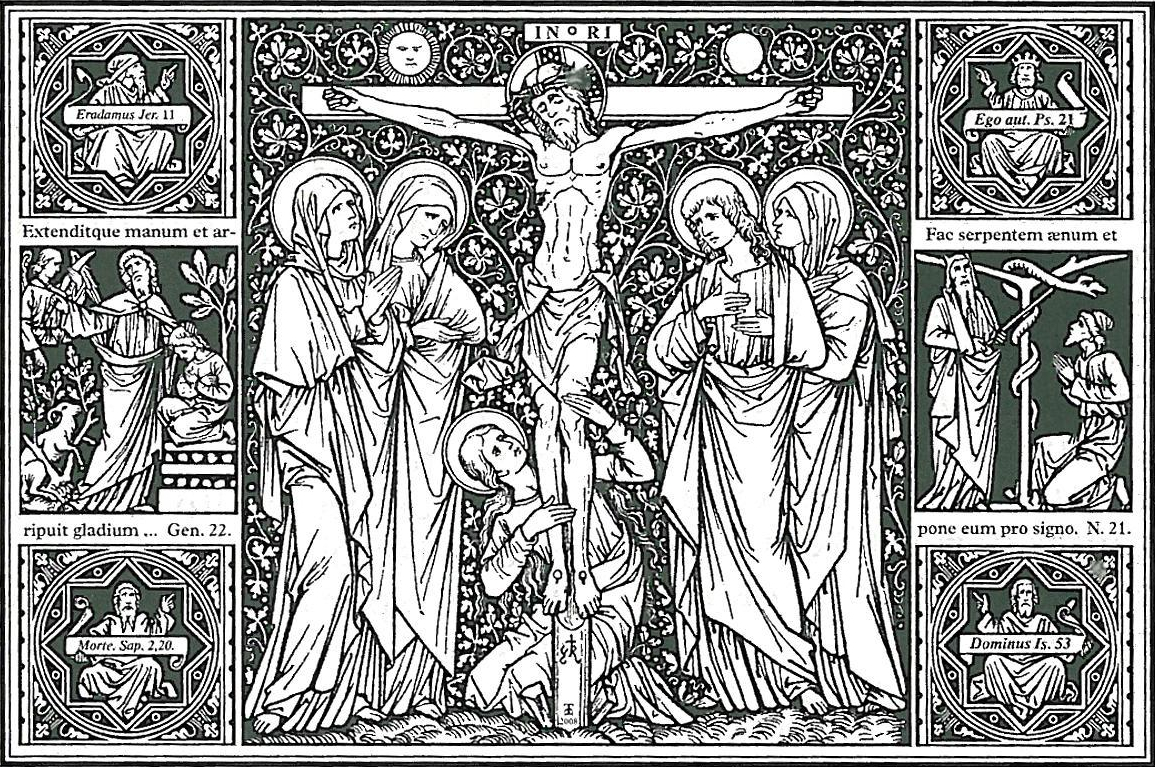
\includegraphics[width=\linewidth]{cross.jpg}
        \end{center}
        %
        % \vfill
        %
        \lettrine[lines=3,depth=1]{\color{Maroon}Q}{\bfseries\color{Maroon}ui}
        pridie quam pateretur, accepit panem in~sanctas ac~venerabiles manus
        suas, et~elevatis oculis in~caelum ad~te Deum Patrem suum omnipotentem,
        tibi gratias agens, bene\krzyz dixit, fregit, deditque discipulis suis,
        dicens: Accipite, et~manducate ex~hoc omnes:\\

        \bigskip

        \centerline{\begin{minipage}{0.75\linewidth}
                \begin{center}
                    \Large\color{Maroon}\bfseries\scshape
                    %
                    Hoc est enim Corpus meum.
                \end{center}
            \end{minipage}}

        \bigskip

        \initial{S}{imili} modo postquam coenatum est, accipiens et~hunc
        praeclarum Calicem in~sanctas ac~venerabiles manus suas: item tibi
        gratias agens, bene\krzyz dixit, deditque discipulis suis, dicens:
        Accipite, et~bibite ex~eo omnes:\\

        \bigskip

        \centerline{\begin{minipage}{0.75\linewidth}
                \begin{center}
                    \Large\color{Maroon}\bfseries\scshape
                    %
                    Hic est enim Calix Sanguinis mei, novi et~aeterni
                    testamenti: mysterium fidei: qui pro vobis et~pro multis
                    effundetur in~remissionem peccatorum.
                \end{center}
            \end{minipage}}

        \bigskip

        \centerline{\begin{minipage}{\linewidth}
                Haec quotiescumque feceritis, in~mei memoriam facietis.
            \end{minipage}}

    \end{minipage}
    \hspace*{0.8cm}
    \begin{minipage}[t]{0.29\linewidth}

        \vspace*{2.2cm}

        \initial{S}{uscipe}, sancte Pater, omnipotens aeterne Deus, hanc
        immaculatam hostiam, quam ego indignus famulus tuus offero tibi Deo meo
        vivo et~vero, pro innumerabilibus peccatis, et~offensionibus, et
        negligentiis meis, et~pro omnibus circumstantibus, sed et~pro omnibus
        fidelibus Christianis vivis atque defunctis: ut~mihi, et~illis proficiat
        ad~salutem in~vitam aeternam. \amen

        \gap

        \initial{O}{fferimus} tibi, Domine, calicem salutaris, tuam deprecantes
        clementiam: ut~in~conspectu divinae majestatis tuae, pro nostra, et
        totius mundi salute cum odore suavitatis ascendat. \amen

        \gap

        \initial{I}{n} spiritu humilitatis, et~in~animo contrito suscipiamur a
        te, Domine: et~sic fiat sacrificium nostrum in~conspectu tuo hodie, ut
        placeat tibi, Domine Deus

        \gap

        \initial{V}{enite}, Sanctificator omnipotens aeterne Deus, et~bene\krzyz
        dic hoc sacrificium, tuo sancto nomini praeparatum.

        \gap

        \initial{S}{uscipe}, sancta Trinitas, hanc oblationem, quam tibi
        offerimus ob memoriam passionis, resurrectionis, et~ascensionis Jesu
        Christi Domini nostri: et~in~honorem beatae Mariae semper Virginis, et
        beati Joannis Baptistae, et~sanctorum Apostolorum Petri et~Pauli, et
        istorum, et~omnium Sanctorum: ut~illis proficiat ad~honorem, nobis autem
        ad~salutem: et~illi pro nobis intercedere dignentur in~caelis, quorum
        memoriam agimus in~terris. Per eumdem Christum Dominum nostrum. \amen

        \gap

        \initial{P}{laceat} tibi, sancta Trinitas, obsequium servitutis meae: et
        praesta; ut~sacrificium quod oculis tuae majestatis indignus obtuli,
        tibi sit acceptabile, mihique, et~omnibus, pro quibus illud obtuli, sit,
        te miserante, propitiabile. Per~Christum Dominum nostrum. \amen

    \end{minipage}
\end{center}

% \vspace*{1cm}

\end{document}
